% Pedagogical schematic: eddy-current induction by an AC coil (meridional view).
\documentclass[border=2pt]{standalone}
% ======================================================================
% tikz-common.tex - shared setup for all standalone figures.
% \input this from the preamble of every figures/fig_*.tex.
% ======================================================================

\usepackage{amsmath,bm}
\usepackage{siunitx}
\usepackage{tikz}
\usetikzlibrary{arrows.meta, calc, positioning, patterns, shapes.geometric,
                decorations.pathmorphing, decorations.pathreplacing}
\usepackage{pgfplots}
\pgfplotsset{compat=1.18}
\usepgfplotslibrary{groupplots, colormaps}

% ---- Okabe-Ito colorblind-safe palette --------------------------------
\definecolor{oiBlue}{RGB}{0,114,178}
\definecolor{oiOrange}{RGB}{230,159,0}
\definecolor{oiGreen}{RGB}{0,158,115}
\definecolor{oiVermillion}{RGB}{213,94,0}
\definecolor{oiSky}{RGB}{86,180,233}
\definecolor{oiPurple}{RGB}{204,121,167}
\definecolor{oiYellow}{RGB}{240,228,66}

\pgfplotscreateplotcyclelist{oi}{%
  {oiBlue,       mark=*,         mark size=1.6pt},
  {oiOrange,     mark=square*,   mark size=1.5pt},
  {oiGreen,      mark=triangle*, mark size=1.9pt},
  {oiVermillion, mark=diamond*,  mark size=1.8pt},
  {oiSky,        mark=pentagon*, mark size=1.7pt},
}

% Axis sized for a single column: 76 mm + labels ~ 86 mm total width.
% NOTE: the default legend sits *below* the axis. This is deliberate -- a legend
% inside the axis box routinely lands on top of lines and markers, and judging
% "which corner is free" by eye is unreliable. Parking it outside the data region
% guarantees no overlap. Override per-figure with the named styles below only
% when a corner is provably empty.
\pgfplotsset{
  every axis/.append style={
    width=76mm, height=57mm,
    line width=0.5pt,
    tick style={line width=0.4pt, black},
    grid=major,
    grid style={gray!25, very thin},
    cycle list name=oi,
    legend cell align=left,
    legend style={
      draw=gray!50, fill=white, font=\footnotesize, inner xsep=3pt,
      % default: centered just below the axis, never over the data
      at={(0.5,-0.30)}, anchor=north,
      legend columns=-1,            % single row; use `legend below columns=N' if too wide
      /tikz/every even column/.append style={column sep=6pt},
    },
    label style={font=\small},
    tick label style={font=\footnotesize},
  },
}

% ---- Named legend-placement overrides ---------------------------------
% The default (above) is already overlap-proof. Use these only to relocate the
% legend deliberately; `legend inside' is the ONLY option that risks covering
% data, so reach for it solely when a corner is demonstrably empty.
\pgfplotsset{
  % Stack entries below the axis in N columns (for many series). Usage:
  %   legend below columns=2
  legend below/.style={
    legend style={at={(0.5,-0.30)}, anchor=north, legend columns=-1},
  },
  legend below columns/.style={
    legend style={at={(0.5,-0.30)}, anchor=north, legend columns=#1},
  },
  % Park the legend to the right of the axis (widens the figure ~15 mm).
  legend right/.style={
    legend style={at={(1.02,1)}, anchor=north west, legend columns=1},
  },
  % Opt back IN to a legend inside the axis box. ONLY when the named corner is
  % provably free of lines and markers. Usage: legend inside corner=north east
  legend inside/.style={
    legend style={at={(0.98,0.98)}, anchor=north east, legend columns=1},
  },
  legend inside corner/.style={
    legend style={legend columns=1},
    legend pos=#1,
  },
}

% Backward-compatible alias for the earlier `legend outside' name.
\pgfplotsset{legend outside/.style={legend right}}

% ---- Flowchart / schematic styles --------------------------------------
\tikzset{
  block/.style={draw, rounded corners=2pt, align=center,
                minimum height=2.4em, inner xsep=7pt, inner ysep=4pt},
  decision/.style={draw, diamond, aspect=2.2, align=center, inner sep=1.5pt},
  io/.style={draw, trapezium, trapezium left angle=70,
             trapezium right angle=110, align=center, inner xsep=6pt},
  flow/.style={-{Latex[length=2.2mm]}},
  dim/.style={{Latex[length=1.8mm]}-{Latex[length=1.8mm]}},
}

\begin{document}
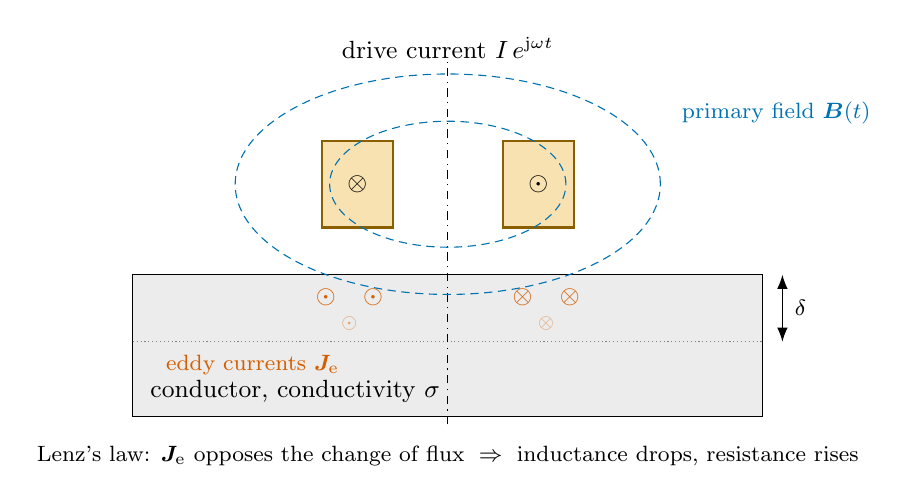
\begin{tikzpicture}[font=\small, x=1cm, y=1cm]
  % conductor
  \fill[gray!15] (0,-1.8) rectangle (8,0);
  \draw (0,-1.8) rectangle (8,0);
  \node[anchor=south west] at (0.1,-1.75) {conductor, conductivity $\sigma$};
  % skin-depth band
  \draw[densely dotted, gray] (0,-0.85) -- (8,-0.85);
  \draw[dim] (8.25,-0.85) -- (8.25,0)
    node[midway, right=1pt, font=\footnotesize] {$\delta$};
  % symmetry axis
  \draw[dash dot, thin] (4,-1.9) -- (4,2.7);
  % coil winding cross-sections: left current into page, right out of page
  \fill[oiOrange!30] (2.4,0.6) rectangle (3.3,1.7);
  \fill[oiOrange!30] (4.7,0.6) rectangle (5.6,1.7);
  \draw[oiOrange!60!black, thick] (2.4,0.6) rectangle (3.3,1.7);
  \draw[oiOrange!60!black, thick] (4.7,0.6) rectangle (5.6,1.7);
  \node at (2.85,1.15) {$\otimes$};
  \node at (5.15,1.15) {$\odot$};
  \node[anchor=south] at (4,2.62) {drive current $I\,e^{\mathrm{j}\omega t}$};
  % primary field loops
  \draw[oiBlue, densely dashed] (4,1.15) ellipse (2.7 and 1.4);
  \draw[oiBlue, densely dashed] (4,1.15) ellipse (1.5 and 0.8);
  \node[oiBlue, anchor=west, font=\footnotesize] at (6.85,2.05)
    {primary field $\bm B(t)$};
  % induced eddy currents near the surface, fading with depth
  \node[oiVermillion] at (2.45,-0.28) {$\odot$};
  \node[oiVermillion] at (3.05,-0.28) {$\odot$};
  \node[oiVermillion, opacity=0.5, scale=0.8] at (2.75,-0.62) {$\odot$};
  \node[oiVermillion] at (4.95,-0.28) {$\otimes$};
  \node[oiVermillion] at (5.55,-0.28) {$\otimes$};
  \node[oiVermillion, opacity=0.5, scale=0.8] at (5.25,-0.62) {$\otimes$};
  \node[oiVermillion, anchor=west, font=\footnotesize] at (0.3,-1.15)
    {eddy currents $\bm J_{\mathrm e}$};
  % Lenz note
  \node[anchor=north, align=center, font=\footnotesize] at (4,-2.05)
    {Lenz's law: $\bm J_{\mathrm e}$ opposes the change of flux
     $\;\Rightarrow\;$ inductance drops, resistance rises};
\end{tikzpicture}
\end{document}
